\chapter{Instalación de GestiONG}

\section{Instalación}
Dependiendo de la distribución de GNU/Linux que utilices, la
instalación de GestiONG será diferente. Si tienes un PC con
\textstylenombreprograma{Debian}, \textstylenombreprograma{Ubuntu} (o
alguna de sus variedades como \textstylenombreprograma{Kubuntu},
\textstylenombreprograma{Xubuntu}, ... ),
\textstylenombreprograma{Fedora}, \textstylenombreprograma{Red Hat} o
\textstylenombreprograma{Mandriva}, estás de enhorabuena porque
GestiONG proporciona paquetes preparados para su instalación de forma
sencilla. Para otras distribuciones, otros tipos de ordenador (como los
Mac) u ordenadores muy antiguos, necesitarás construir el programa
tú misma.

\subsection{Usando paquetes preparados para tu sistema}
En la página de descarga del proyecto,
\href{http://sourceforge.net/project/showfiles.php?group_id=80104&package_id=81685&release_id=578703}{https://sourceforge.net/project/showfiles.php?group\_id=80104}
encontrarás una lista de paquetes disponibles para distintas
arquitecturas de computadoras y distribuciones de GNU/Linux. 



\begin{center}
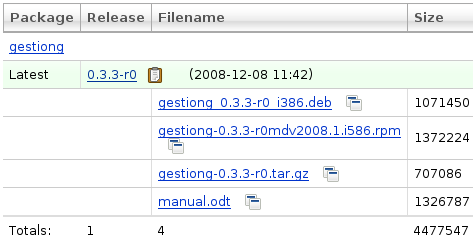
\includegraphics[width=7.915cm,height=4.166cm]{manual-img1.png}
\captionof{figure}[Zona de descarga desde sourceforge.net]{Zona de
descarga desde sourceforge.net}

\end{center}
Haz click sobre el fichero correspondiente a tu distribución: para
\ \textstylenombreprograma{Fedora}, \textstylenombreprograma{Mandriva}
y \textstylenombreprograma{Red Hat}, elige:

\ \ \ \textstyleGUIELEMENT{gestiong-0.3.3-r0mdv2008.1.i586.rpm.}

Para \textstylenombreprograma{Debian},
\textstylenombreprograma{K/Ubuntu} y
\textstylenombreprograma{Guadalinex,} elige:

\textstyleGUIELEMENT{\ \ gestiong\_0.3.3-r0-1\_i386.deb. }

Para el resto, elige: 

\textstyleGUIELEMENT{\ \ \ \ gestiong-0.3.3-r0.tar.gz} 

y salta al apartado: \textit{Construyendo el programa}. 


\bigskip


\bigskip

Si tu distribución y tu navegador de Internet son lo suficientemente
modernas, te aparecerá una serie de ventanas para realizar la
instalación automática. Por ejemplo, con Firefox y Mandriva:



\begin{center}
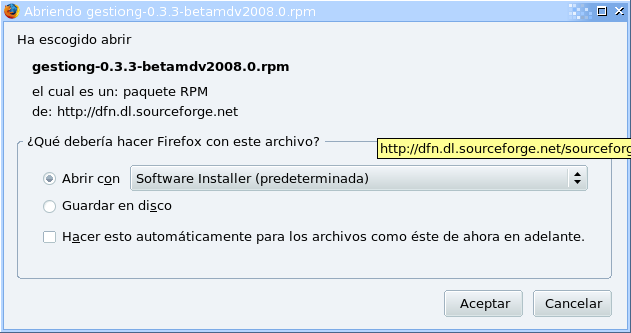
\includegraphics[width=7.964cm,height=4.643cm]{manual-img2.png}
\end{center}
\begin{center}
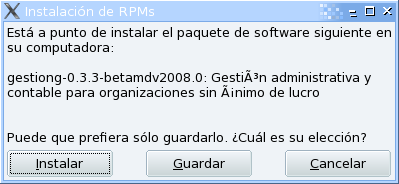
\includegraphics[width=8.345cm,height=3.928cm]{manual-img3.png}
\end{center}
\begin{center}
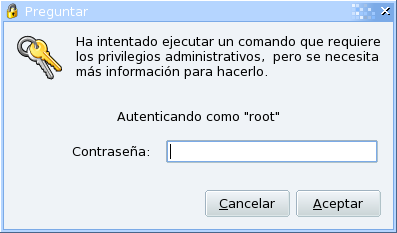
\includegraphics[width=7.758cm,height=4.648cm]{manual-img4.png}
\end{center}
\begin{center}
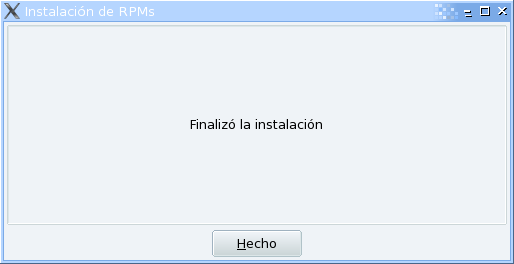
\includegraphics[width=8.56cm,height=4.489cm]{manual-img5.png}
\end{center}

\bigskip


\bigskip


\bigskip


\bigskip


\bigskip


\bigskip


\bigskip


\bigskip



\begin{center}
\begin{minipage}{16.919cm}
{\centering\bfseries\itshape
\label{ref:accesoroot}Acceso a root
\par}

En los sistemas operativos multiusuaria del tipo GNU/Linux hay una
usuaria especial llamada \textbf{\textit{root}} que tiene permiso para
hacerlo todo. Puede instalar y eliminar programas, agregar y quitar
hardware, acceder a cualquier fichero y en general realizar cualquier
tarea administrativa. El resto de usuarias tiene un conjunto de
permisos más reducido, por lo que para ciertas operaciones necesitan
acceder al ordenador como \textbf{\textit{root}}, y por lo tanto deben
conocer su contraseña o bien pedir a la usuaria
\textbf{\textit{root}} que realice esas operaciones.

En la consola las órdenes \textbf{sudo} y \textbf{su} sirven para
ejecutar comandos como si fueras \textbf{root}, preguntando previamente
su contraseña, como verás más adelante.
\end{minipage}
\end{center}
En caso de no instalarse automáticamente, guarda el paquete en tu
carpeta de inicio o personal (o {\textquotesingle}Home
Folder{\textquotesingle}), abre una consola (lee el recuadro !`Abre una
consola! en la página \pageref{ref:abreunaconsola}), y dependiendo de
tu distribución:

{\bfseries\itshape
Mandriva, Fedora y Red Hat:}



\begin{center}
\begin{minipage}{16.48cm}
\textstyleUserEntry{\$ cd}

\textstyleUserEntry{\$ su}

\textstyleUserEntry{password:}\textstyleUserEntry{
\ \ }\textstylekonsolecomment{(escribe la contraseña de root y pulsa
Intro, ATENCION: NO SE VERÁ LO QUE ESCRIBAS)}

\textstyleUserEntry{\# rpm -ihv
}\textstyleUserEntry{gestiong-0.3.3-r0mdv2008.0.rpm}

\textstyleUserEntry{\$ exit}
\end{minipage}
\end{center}

\bigskip


\bigskip


\bigskip

{\bfseries\itshape
Debian, Ubuntu, Kubuntu, GuadaLinex.}



\begin{center}
\begin{minipage}{16.48cm}
\textstyleUserEntry{\$ cd}

\textstyleUserEntry{\$ sudo dpkg -i
}\textstyleUserEntry{gestiong\_0.3.3-r0\_i386.deb}

\textstyleUserEntry{password:}\textstyleUserEntry{
\ \ }\textstylekonsolecomment{(escribe la contraseña de root y pulsa
Intro, ATENCION: NO SE VERÁ LO QUE ESCRIBAS)}
\end{minipage}
\end{center}
Si todo ha funcionado correctamente, lee el apartado Creando un enlace a
GestiONG en el escritorio en la página \pageref{ref:creaenlace}.

\subsection{Construyendo el programa}
\label{ref:construyendoprograma}Si no hay paquetes disponibles para tu
sistema o no están actualizados, puedes construir tú misma el
programa a partir de sus fuentes. Si sabes cómo hacerlo, estas son
las instrucciones:



\begin{center}
\begin{minipage}{16.48cm}
\textstyleUserEntry{\$ cd}

\textstyleUserEntry{\$ mkdir gongsrc}

\textstyleUserEntry{\$ cd gongsrc}

\textstyleUserEntry{\$ wget
}\href{http://dfn.dl.sourceforge.net/sourceforge/gestiong/gestiong-0.3.3-alfa.tar.gz}{\textstyleUserEntry{http://dfn.dl.sourceforge.net/sourceforge/gestiong/gestiong-0.3.3-r0.tar.gz}}

\textstyleUserEntry{\$ tar -zxvf gestiong-0.3.3-r0.tar.gz}

\textstyleUserEntry{\$ cd gestiong-0.3.3}

\textstyleUserEntry{\$ ./configure -{}-prefix=/usr/local}

\textstyleUserEntry{\$ make}

\textstyleUserEntry{\$ sudo make install}

\textstyleUserEntry{\$ gestiong}
\end{minipage}
\end{center}

\bigskip


\bigskip


\bigskip


\bigskip


\bigskip


\bigskip


\bigskip

Dependiendo de tu familiaridad con GNU/Linux puedes entender o no este
proceso, pero aún sin entender nada, siguiendo las instrucciones a
continuación deberías ser capaz de construirlo. Si estás
totalmente perdida, es absolutamente necesario que leas primero el
recuadro \textit{!`Abre una consola!}. 

\begin{center}
\begin{minipage}{16.947cm}
{\centering\bfseries\itshape
\label{ref:abreunaconsola}!`Abre una consola!
\par}

En el mundo de GNU/Linux, todas las operaciones de administración del
ordenador (instalar programas, instalar una impresora, añadir
usuarias, configurar el acceso a Internet, hacer copias de seguridad,
etc.) se pueden realizar tanto con programas gráficos (con botones,
colores y usando el ratón) como tecleando comandos desde una ventana
con fondo negro y letras blancas (o viceversa) conocida como \textit{la
consola}. No es necesario conocer estos comandos para utilizar un
sistema GNU/Linux, pero en algún momento de tu vida alguien te
dirá: {\textquotedblleft}\textit{Abre una
consola}{\textquotedblright} y entrarás de lleno en el mundo del
hacking.

Dependiendo del escritorio que utilices la abrirás de una forma
distinta. Para \textbf{\textit{Gnome}}, pulsa
\textstyleGUIELEMENTREDUCED{Alt+F2 }y escribe \textbf{gnome-terminal} y
pulsa \textstyleGUIELEMENTREDUCED{Intro} (o elige desde el menú
principal: \textstyleGUIELEMENTREDUCED{Aplicaciones$\rightarrow
$Accesorios$\rightarrow $Terminal}).\textstyleGUIELEMENTREDUCED{ }En
KDE, pulsa \textstyleGUIELEMENTREDUCED{Alt+F2} \ (o elige la opción
{\textquotesingle}\textstyleGUIELEMENTREDUCED{Ejecutar
orden}{\textquotesingle} del menú principal), escribe
\textbf{konsole} y pulsa \textstyleGUIELEMENTREDUCED{Intro}. 



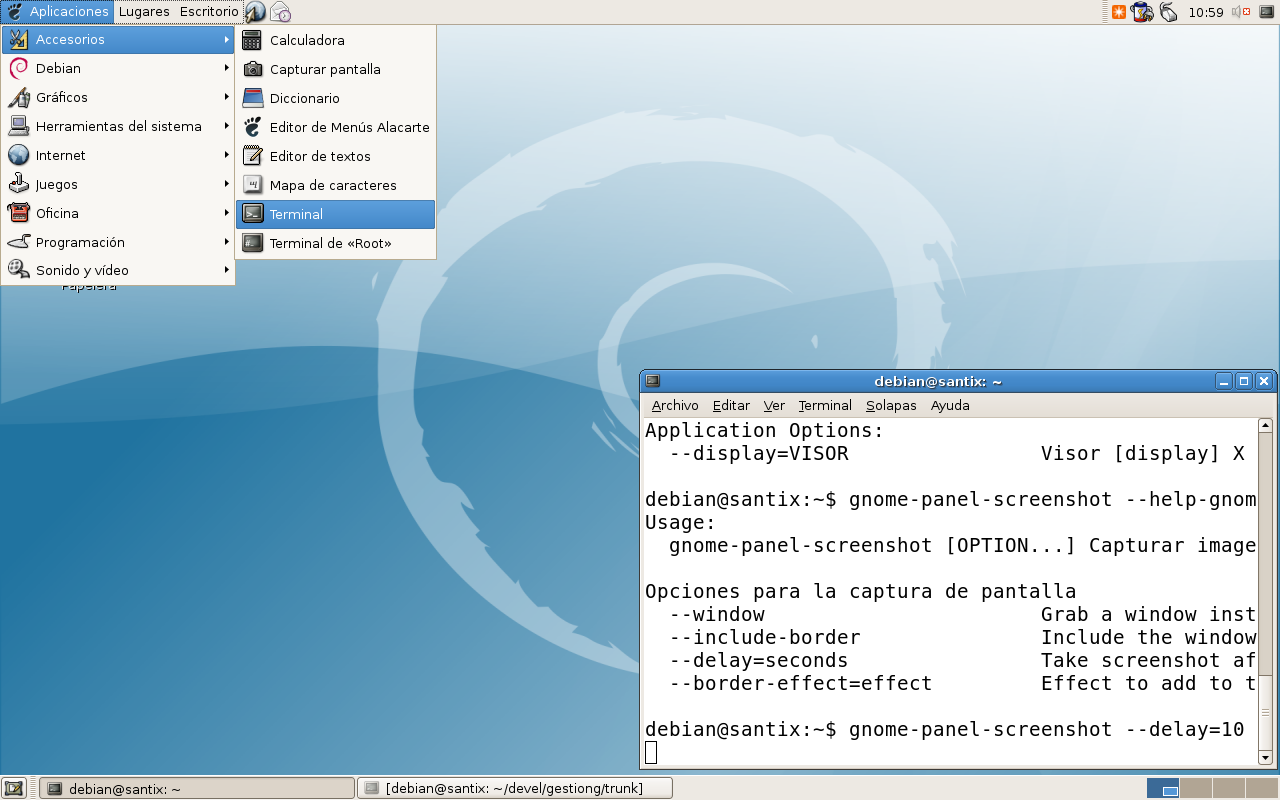
\includegraphics[width=7.915cm,height=4.946cm]{manual-img6.png}
\captionof{figure}[El escritorio de Gnome]{El escritorio de Gnome}
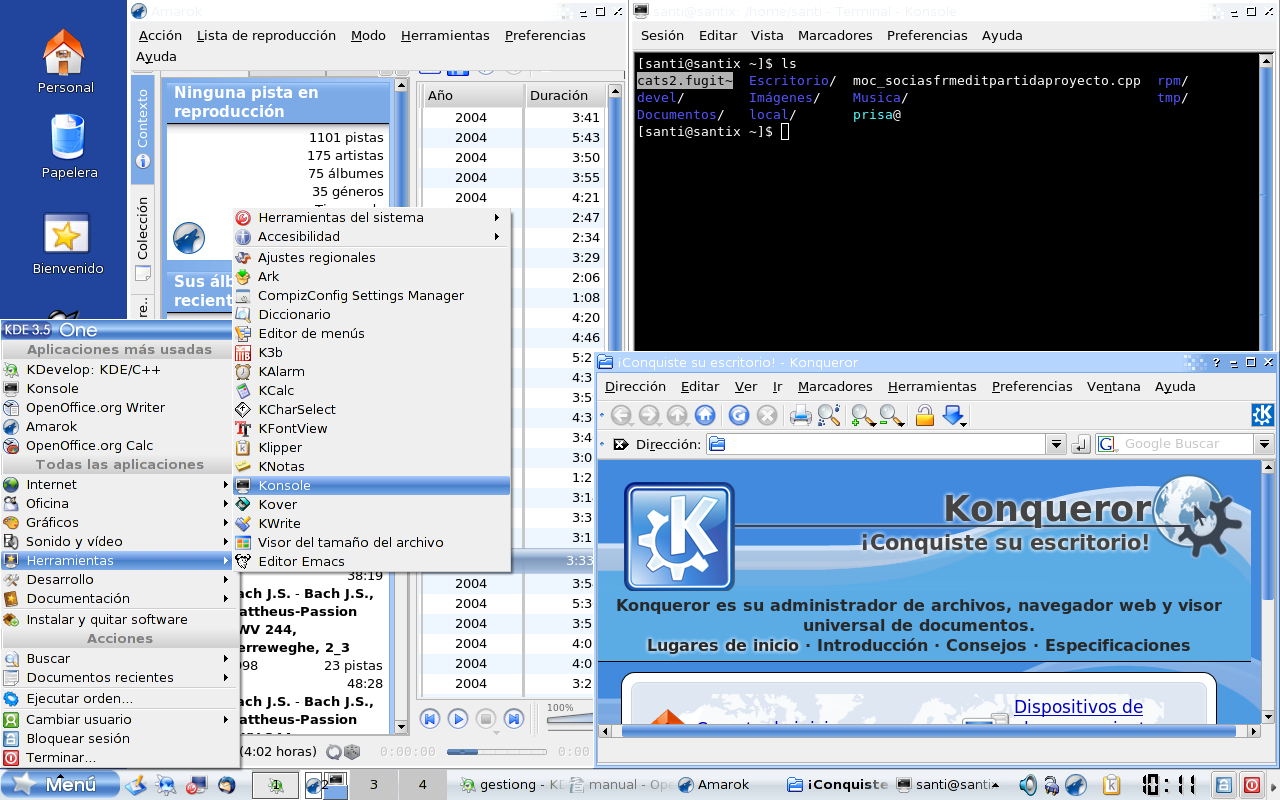
\includegraphics[width=7.953cm,height=4.868cm]{manual-img7.png}
\captionof{figure}[El escritorio de KDE]{El escritorio de KDE}
En la consola estableces una comunicación con el ordenador, a su
manera. Éste presenta una línea acabada con un símbolo de dólar
y un cursor parpadeante donde puedes escribir órdenes o comandos.
Cada vez que escribas una orden \textbf{debes pulsar}
\textstyleGUIELEMENTREDUCED{Intro} para que el ordenador la interprete
y muestre el resultado o un mensaje de error. Escribe la orden
\textbf{ls} (una ele y una ese) y pulsa
\textstyleGUIELEMENTREDUCED{Intro }y observa lo que aparece. Ahora
escribe \textbf{cmderroneo} y observa el mensaje de error. Cuando
quieras cerrar la consola, escribe el comando \textbf{exit}.

Ya estás preparada para realizar cualquier operación desde la
consola. En este manual, los comandos que necesitas ejecutar en una
consola se mostrarán dentro de un cuadro como este:

donde se ha suprimido la parte a la izquierda del \$ ya que en cada
ordenador será diferente. Tienes que escribir lo que hay a la derecha
del símbolo de dólar respetando todos los guiones, espacios,
puntos, etc. Si la orden es complicada, siempre puedes copiar y pegar.
Al final de cada línea, pulsa \textstyleGUIELEMENTREDUCED{Intro}.
\begin{minipage}{16.489cm}
\textstyleUserEntry{\$ cd gongsrc \ \ }\textstylekonsolecomment{(Aquí
a la derecha pueden aparecer algunas aclaraciones)}

\textstyleUserEntry{\$ ls }\ \ \textstylekonsolecomment{(que no tienes
que teclear)}
\end{minipage}\end{minipage}
\end{center}
\clearpage\paragraph{Descargando el programa}
Antes de comenzar, mediante la consola, vas a crear una carpeta dentro
de tu carpeta personal o de inicio (o {\textquotesingle}\textit{Home
Folder}{\textquotesingle}) que se llamará
{\textquotesingle}\textit{gongsrc}{\textquotesingle} donde realizarás
todo el proceso de construcción. \textit{!`Abre una consola!} y
teclea lo siguiente: (recuerda que solamente tienes que teclear lo que
hay a la derecha del símbolo del dólar):



\begin{center}
\begin{minipage}{16.48cm}
\textstyleUserEntry{\$ cd}

\textstyleUserEntry{\$ mkdir gongsrc}

\textstyleUserEntry{\$ cd gongsrc}
\end{minipage}
\end{center}

\bigskip

Ahora tienes que conseguir el fichero comprimido que contiene el
código fuente para la versión que vas a instalar:
\textit{gestiong-0.3.3-r0.tar.gz}. Puedes descargarlo con tu navegador
favorito desde la página:

\ \ \url{http://sourceforge.net/project/showfiles.php?group_id=80104&package_id=81685&release_id=578703}



\bigskip

y guardarlo en la carpeta gongsrc que acabas de crear en tu carpeta
personal.


\bigskip

Aunque es más fácil y rápido descargarlo desde la consola
utilizando el comando wget: 



\begin{center}
\begin{minipage}{16.48cm}
\textstyleUserEntry{\$ wget
http://dfn.dl.sourceforge.net/sourceforge/gestiong/gestiong-0.3.3-r0.tar.gz}
\end{minipage}
\end{center}
Independientemente de cómo consigas el fichero, una vez descargado y
grabado en la carpeta
{\textquotesingle}\textit{gongsrc}{\textquotesingle}, tienes que
descomprimirlo con las siguientes órdenes:

\paragraph[]{}
\begin{center}
\begin{minipage}{16.856cm}
\textstyleUserEntry{\$ tar -zxvf
gestiong-0.3.3-r0.tar.gz}\textstyleUserEntry{\ \ }\textstylekonsolecomment{(Aparecerán
muchas letras muy rápidas...)}

\textstyleUserEntry{\$ cd gestiong-0.3.3}
\end{minipage}
\end{center}
\paragraph{Preparando el entorno para la construcción}
Si no has realizado nunca el proceso de construcción de un programa en
tu ordenador, lo más probable es que necesites instalar una serie de
herramientas de programación, para lo cual necesitarás
\textbf{acceso a Internet} y la contraseña de root (ver
recuadro\textit{ }\textit{Acceso a root}\textit{ }en la página
\pageref{ref:accesoroot}):

Según tu distribución, esto es lo que tienes que hacer (recuerda que
necesitas acceso a Internet):



\begin{center}
\begin{minipage}{16.701cm}
{\itshape
\ \ \textstylekonsolecomment{(Para las distribuciones K/Ubuntu/Debian de
GNU/Linux:)}}

\textstyleUserEntry{\$ sudo aptitude install build-essential
libqt3-mt-dev libboost-dev }

\textstyleUserEntry{password:}\textstyleUserEntry{
\ \ }\textstylekonsolecomment{(escribe la contraseña de root y pulsa
Intro, ATENCION: NO SE VERÁ LO QUE ESCRIBAS)}

\textstyleUserEntry{\$ sudo aptitude install libxml2-dev
libmysqlclient15-dev libdb4.5-dev}


\bigskip

{\itshape
\ \ \textstylekonsolecomment{(Para la distribución Mandriva de
GNU/Linux:)}}

\textstyleUserEntry{\$ su}

\textstyleUserEntry{password:}\textstyleUserEntry{
\ \ }\textstylekonsolecomment{(escribe la contraseña de root y pulsa
Intro, ATENCION: NO SE VERÁ LO QUE ESCRIBAS)}

\textstyleUserEntry{\# urpmi make gcc-c++ libqt3-devel libboost1-devel}

\textstyleUserEntry{\# urpmi libxml2-devel libmysql-devel
libdb4.5-devel}

\textstyleUserEntry{\$ exit}

{\itshape
\textstylekonsolecomment{\ \ (Para las distribucies Fedora y Red Hat de
GNU/Linux:)}}


\bigskip
\end{minipage}
\end{center}

\bigskip


\bigskip

\paragraph{Compilando}
Antes de compilar las fuentes del programa, tienes que decidir si lo vas
a instalar en modo local (para una sola usuaria) o en modo global (para
todas las usuarias de tu ordenador). Normalmente lo querrás instalar
en modo global, reservando el modo local para cuando no tienes acceso a
\textit{root}. (Ver el recuadro {\textquotedblleft}\textit{Acceso a
root}{\textquotedblright}).

Si lo vas a instalar globalmente, ejecuta los siguientes comandos (el
comando \textbf{make }tardará bastante y escribirá un montón de
basurilla; sabrás que ha terminado cuando vuelva a aparecer el prompt
\$):



\begin{center}
\begin{minipage}{16.48cm}
\textstyleUserEntry{\$ ./configure }

\textstyleUserEntry{\$ make}

\textstyleUserEntry{\$ sudo make install}

\textstyleUserEntry{password: \ \ }\textstylekonsolecomment{(escribe la
contraseña de root y pulsa Intro, ATENCION: NO SE VERÁ LO QUE
ESCRIBAS)}
\end{minipage}
\end{center}

\bigskip


\bigskip

Si lo vas a instalar localmente:



\begin{center}
\begin{minipage}{16.48cm}
\textstyleUserEntry{\$ ./configure -{}-prefix=\$HOME/local}

\textstyleUserEntry{\$ make}

\textstyleUserEntry{\$ make install}
\end{minipage}
\end{center}

\bigskip


\bigskip


\bigskip

!`Enhorabuena! Ya tienes GestiONG instalado en tu ordenador. Ahora
puedes ponerlo en marcha, pero recuerda que para poder trabajar con
él, necesitas primero instalar la base de datos.

\paragraph{Ejecutando GestiONG}
Dependiendo del tipo de instalación que hayas elegido para GestiONG,
local o global, el programa estará en un lugar distinto. 

En global, ejecuta simplemente:



\begin{center}
\begin{minipage}{16.48cm}
\textstyleUserEntry{\$ \ gestiong}
\end{minipage}
\end{center}

\bigskip

En local, teclea este comando (teclea también el dólar delante de
HOME):



\begin{center}
\begin{minipage}{16.48cm}
\textstyleUserEntry{\$ \ \$HOME/local/bin/gestiong}
\end{minipage}
\end{center}

\bigskip


\bigskip

\subsection{Creando un enlace a GestiONG en el escritorio}
\label{ref:creaenlace}De nuevo aquí, dependiendo de tu distribución
de GNU/Linux, la operación será algo distinta. Pero se puede
reducir básicamente a dos escritorios, KDE y GNOME (si utilizas otro
entorno, seguro que sabes crear el acceso directo).

Haz click con el botón derecho del ratón en un área vacía del
escritorio y:

a) para KDE, selecciona, {\textquotesingle}\textstyleGUIELEMENT{Crear
Nuevo...}{\textquotesingle}
({\textquotesingle}\textstyleGUIELEMENT{Create
New...}{\textquotesingle}) y luego
{\textquotesingle}\textstyleGUIELEMENT{Enlace a
aplicación...}{\textquotesingle}
({\textquotesingle}\textstyleGUIELEMENT{Link to
application...}{\textquotesingle}). Haz click sobre la pestaña
{\textquotesingle}\textstyleGUIELEMENT{Aplicación}{\textquotesingle}
({\textquotesingle}\textstyleGUIELEMENT{Application}{\textquotesingle}).

b) para Gnome: selecciona {\textquotesingle}\textstyleGUIELEMENT{Crear
un lanzador...}{\textquotesingle}
({\textquotesingle}\textstyleGUIELEMENT{Create
New...}{\textquotesingle}).

En el recuadro
{\textquotesingle}\textstyleGUIELEMENT{Comando}{\textquotesingle}
({\textquotesingle}\textstyleGUIELEMENT{Command}{\textquotesingle})
escribe la localización del programa \textit{gestiong}. Si lo has
instalado desde un paquete preparado para tu sistema o lo has
construido globalmente, escribe simplemente \textit{gestiong}. Si lo
has construido en local, escribe \textit{\$HOME/local/bin/gestiong.}
Pulsa el botón
{\textquotesingle}\textstyleGUIELEMENT{Aceptar}{\textquotesingle}
({\textquotesingle}\textstyleGUIELEMENT{Ok}{\textquotesingle}) y ya
tendrás en tu escritorio el enlace a GestiONG.

\clearpage\subsection{Instalando el servidor de la base de datos}
\label{ref:instalandosqlserver}Dependiendo del número y localización
de los ordenadores de tu organización, quizás sea necesario
instalar la base de datos en uno de ellos. Los escenarios más
frecuentes con los que te puedes encontrar son:

\begin{center}
\begin{minipage}{7.687cm}
{\centering\bfseries\itshape
¿Qué es el servidor de la base de datos?
\par}

Los datos con los que trabajan aún muchas asociaciones suelen estar
contenidos en varias hojas de cálculo: la hoja de socias, la de
gastos, etc. lo cual presenta ciertos inconvenientes, como acceso
incontrolado, duplicidad de datos, imposibilidad de actualizaciones
simultáneas, descentralización, etc.

GestiONG usa un sistema de base de datos independiente llamado MySQL
(www.mysql.com), el cual permite entre otras cosas:

\liststyleLiv
\begin{enumerate}
\item almacenamiento centralizado de los datos,
\item el acceso solo a usuarias identificadas,
\item el acceso desde cualquier ordenador conectado a la red local o a
través de Internet,
\item una capacidad prácticamente ilimitada de almacenamiento.
\end{enumerate}
Con GestiONG se pueden gestionar múltiples asociaciones, cada una con
su correspondiente base de datos que pueden estar localizadas en
diversos lugares.
\end{minipage}
\end{center}
\liststyleLv
\begin{enumerate}
\item \begin{enumerate}
\item Si solamente tenéis un ordenador en vuestra asociación,
tendréis que instalar tanto la base de datos como GestiONG en el
mismo ordenador, que actuará como servidor.
\item Si tenéis varios ordenadores conectados en red, solo será
necesario instalar la base de datos en uno de ellos, que asumirá el
papel de servidor y podréis instalar GestiONG en el resto de
ordenadores conectados a aquél.
\item También podéis tener la base de datos fuera de la oficina, por
ejemplo, cuando se instala en la sede central de la organización o
cuando habéis contratado el servicio de base de datos con una empresa
externa. En ese caso, la central o la empresa proveedora os
facilitará la información necesaria para conectar con el servidor.
\end{enumerate}
\end{enumerate}

\bigskip

Para los escenarios a) y b), necesitarás acceso como \textit{root} al
ordenador donde vas a instalar el servidor (lee el recuadro
{\textquotedblleft}\textit{Acceso a root}{\textquotedblright} en la
página \pageref{ref:accesoroot} si no estás familizarizada con este
concepto). \textit{!`Abre una consola!} en ese ordenador y ejecuta lo
siguiente:



\begin{center}
\begin{minipage}{16.48cm}
{\itshape
\textstylekonsolecomment{\ \ (Para las distribuciones K/Ubuntu/Debian de
GNU/Linux:)}}

\textstyleUserEntry{\$ sudo apt-get install mysql-server}

{\itshape
\textstylekonsolecomment{\ \ (Para la distribución Mandriva de
GNU/Linux:)}}

{\itshape
\textstyleUserEntry{\textup{\$ su}}}

{\itshape
\textstyleUserEntry{\textup{\$ urpmi mysql}}}
\end{minipage}
\end{center}

\bigskip


\bigskip

Ahora, pon una contraseña a la superusuaria del servidor de la base de
datos (sustituye el texto \ \textit{tunuevacontraseña} por la
contraseña que quieres poner):



\begin{center}
\begin{minipage}{16.48cm}
\$ mysqladmin password \textit{tunuevacontraseña}
\end{minipage}
\end{center}

\bigskip


\bigskip

Si has optado por el escenario b), necesitas saber la dirección IP de
este ordenador, conocido como \textit{servidor de la base de datos}.
Ejecuta este comando \ y anota los cuatro números que aparecen tras
\textbf{inet addr:}, algo así \ como 192.168.1.120.



\begin{center}
\begin{minipage}{16.48cm}
\textstyleUserEntry{\$ su}

\textstyleUserEntry{\# ifconfig eth0 {\textbar} grep
{\textquotedblleft}inet addr{\textquotedblright} {\textbar} grep -v
127{\textbackslash}.}

\textstyleUserEntry{\# exit}
\end{minipage}
\end{center}

\bigskip


\bigskip

Recuerda estos datos para cuando tengas que crear la base de datos de
GestiONG más adelante: para los escenarios a) y b) la contraseña
que has puesto a la superusuaria; para el escenario b) además, la
dirección IP del servidor donde has instalado MySQL; para el
escenario c), esta información te la proporcionarán externamente. 
